\documentclass[paper=A4,bibliography=totocnumbered]{scrartcl}
\setkomafont{disposition}{\normalcolor\bfseries} %in KOMA headings are default sans serif, with this patch with serifs see scrguide.pdf, 2010-09-14, page 108
\usepackage[dvipsnames]{xcolor}
\usepackage[latin1]{inputenc} % correct coding for windows e.g. with umlauts
\usepackage[T1]{fontenc}
\usepackage{paralist} % compactenum and compactitem
\usepackage[pdftex]{graphicx} % required to insert figures
\usepackage{listings} % format code
\lstset{escapeinside={<@}{@>}}
\usepackage[margin=10pt,font=small,labelfont=bf,labelsep=endash,singlelinecheck=false,format=plain]{caption} % formatting of captions
\usepackage{booktabs} %for professional tables using \toprule, \midrule, \bottomrule
\usepackage[round]{natbib} % http://merkel.zoneo.net/Latex/natbib.php for author-year citation with round brackets
\usepackage{vmargin} % for margins, especially bottommargin smaller, alternative to DIV=12
\setmarginsrb{35mm}{20mm}{25mm}{15mm}{12pt}{11mm}{0pt}{11mm}

% math packages
\usepackage{amsmath}
\usepackage{amssymb}
\usepackage{centernot}
\usepackage{leftidx}

% set up chapter depths
\newcommand{\subsubsubsection}[1]{\paragraph{#1}\mbox{}\\}
\setcounter{secnumdepth}{4}
\setcounter{tocdepth}{4}
\usepackage{subfig}
\usepackage[hidelinks]{hyperref} % linked pdf, necessarily at the end of preamble!!!

%##########################################################
%###################### Help! #############################
%##########################################################
% 
% Strg+T to comment a block 
% 
% \citet --> Mustermann et al. (2042)
% \citet* --> Mustermann, Musterfrau and Musterkind (2042)
% \citep --> (Mustermann et al. 2042)
% \citep* --> (Mustermann, Musterfrau and Musterkind 2042)
% 
% Insert a picture called xxx.png which is stored in the folder pic as a png
%\begin{figure}
%	\centering
%	\includegraphics[width=13cm]{pic/xxx}
%	\caption[Short Title]{Caption insert here}
%	\label{fig:somelabelname}
%\end{figure}
%
%##########################################################
%########### End Preferences, Begin Document ##############
%##########################################################

%opening
\title{Programming Project 03}
\author{Franc�l Lamprecht, Christine Robinson, Regina Wehler}
\date{Winter Semester 2018/19}

\begin{document}

\maketitle

\tableofcontents
\clearpage
\section{Introduction}
This is a dummy sentence that shows how citations work \citep{Adams.2018}.


\section{Methodology}
The image analysis approach consists of three main steps (figure \ref{fig:pipeline}). First, the input RGB input image is segmented into two class, plant and background by a trainable Weka segmentation classifier. Second, the binary class output is used to identify single leaf objects by watershed segmentation. The resulting binary mask is utilized to analyze properties of the leaf objects in the single red, green and blue channel, respectively.

\begin{figure}
	\centering
	\subfloat[Input]{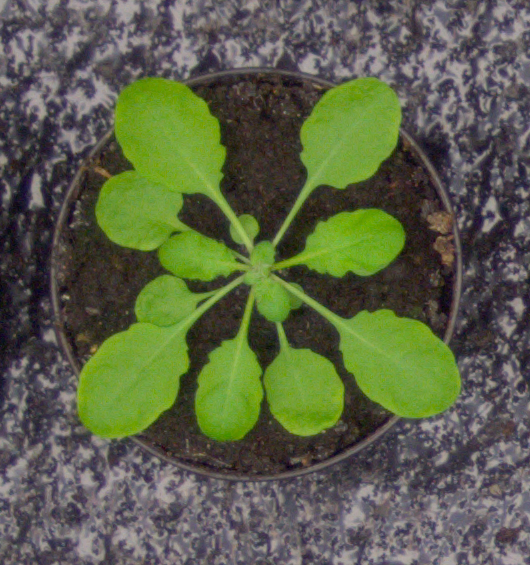
\includegraphics[width=.3\textwidth]{pic/27_rgb}}
	\qquad
	\subfloat[Classification]{
\includegraphics[width=.3\textwidth]{pic/27_class}}
	\qquad
	\subfloat[Watershed]{
\includegraphics[width=.3\textwidth]{pic/27_watershed}}
	\qquad
	\subfloat[Particle Analysis]{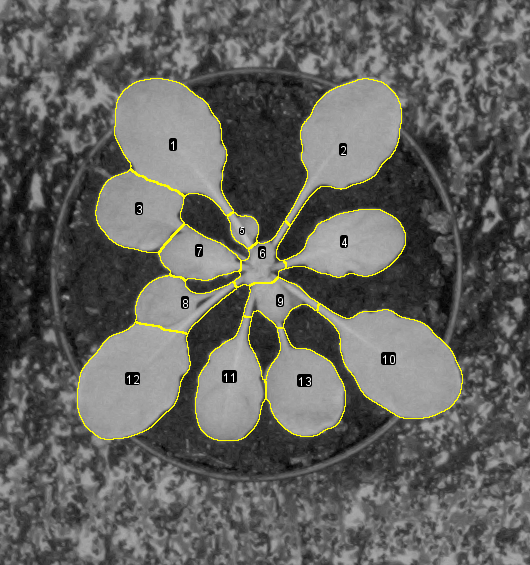
\includegraphics[width=.3\textwidth]{pic/27_greenPA}}
	\caption[Image analysis pipeline]{The analysis of plant leaves is conducted in three steps. The RGB input image (a) is classified into plant and background by a trainable Weka segmentation classifier (b). Single leaf objects are identified by watershed segmentation (c). The binary mask is used to analyze properties in the split red, green and blue channel (d).}
	\label{fig:pipeline}
\end{figure}

\subsection{Segmentation}
The plant is separated from the background with the help of a trainable Weka segmentation classifier, which is available as a plugin for Fiji. The trainable Weka segmentation provides a GUI to train machine learning algorithms to produce pixel-based segmentations. The user can add traces to classes and after classifier training, traces/regions of interest can be adjusted to improve classification. Six representative pictures are selected from the 2017 data set to train the classifier (plant029, plant145 and plant159 from A1; plant032, plant034 and plant037 from A2). Pictures are chosen to cover the whole range of plant green shades and the range of background characteristics. The Weka Experimenter was used to assess the performance of different machine learning algorithms. Based on these results (table \ref{tab:weka}), FastRandomForest was used as a classifier. 

\begin{table}[htbp]
	\centering
	\caption{Comparison of classifier performance by Weka Experimenter. The default algorithm parameters were kept.}
	\begin{tabular}{lllllll}
		\toprule
		Algorithm & Percent correct & Precision & Recall & F score & Matthews  & AUC \\
		 & & & & & correlation & \\
		 \midrule
		FastRandomForest & 99.93 & 1.00 & 1.00 & 1.00 & 1.00 & 1.00 \\
		SMO   & 92.52 & 0.89 & 0.93 & 0.91 & 0.85 & 0.93 \\
		$k$-nearest Neighbors   & 95.38 & 0.95 & 0.93 & 0.94 & 0.90 & 0.95 \\
		RandomSubSpace & 99.85 & 1.00 & 1.00 & 1.00 & 1.00 & 1.00 \\
		Bagging & 99.77 & 1.00 & 1.00 & 1.00 & 1.00 & 1.00 \\
		DesicisonTable & 99.05 & 0.99 & 0.9 & 0.99 & 0.98 & 1.00 \\
		\bottomrule
	\end{tabular}
	\label{tab:weka}
\end{table}


\subsection{Object Recognition}
Watershed 

\subsection{Object Analysis}
Particle Analyzer and additional stuff until csv export

\subsection{Explorative Data Analysis}
Everything in Python

\section{Results}


\section{Discussion \& Outlook}


\renewcommand\bibname{References} % necessarily before \bibliography{ref}, but not working in preamble
\bibliographystyle{apalike} % for references chapter
\bibliography{ref}

\end{document}
